\chapter{System Design}
\section{System Architecture}
\subsection{Logical Architecture}
We are using the m´Meteor framework in this project, and Meteor in turn uses the open source database, MongoDB, which is different from traditional SQL databases like MySQL, Postgresql and OracleDB. MongoDB is NoSQL type database. Meteor uses MongoDB in a very unique way to achieve real-time update of view layer.

Traditionally when users interact with something on the view layer, for instance, clicking on log in or sign up button, the action triggers interaction with database sitting on the server side. This kind of interaction with the database often results in reloading of the page the user is currently on. Not only the reloading of the page is a bad user experience, it ‘eats’ bandwidth and network data because reloading of a page reloads the whole page when only a part of the page is needed to be updated.

Meteor’s way to solve this problem is by creating a mini replica of the MongoDB database on the client side. In this mini-Mongo database, partial data that users need to interact, are stored. Since mini-Mongo database resides on the user side, interactions happen in real time which means data is updated almost constantly without the page needing to reload at all. This feature enables smooth interaction on the view layer and users do not need to wait long for a response from the server. To better illustrate this feature, please see the below diagram for the overall architecture of Meteor framework. 

\subsection{Physical Deployment}
\section{System Components}
\subsection{Data Model}
Our solution has three main entities. These are users, events and exercises. Events can be created by both users and administrators, they are fixed to certain dates and times, and creators of events can invite friends to these events. Exercises, on the other hand, are urls pointing to exercise videos. They are not fixed to any date or location, nor can one invite friends to join exercises. Exercises can only be added to the system by administrators. Exercises can also be included in events, but not vise versa. Figure XX describes the data model and shows how the different entities are related.

//TODO: burde vi oppdatere modellen?
\subsection{Class Diagrams}
\subsection{Sequence Diagrams??}
\subsection{State Diagram of Web Solution}
Below follows a state diagram of the web solution, displaying which pages can be reached by which pages and through which methods. The differently colours lines indicate which pages are available to all users and which only available once users are logged-in. 
\begin{figure}[H]
\centering
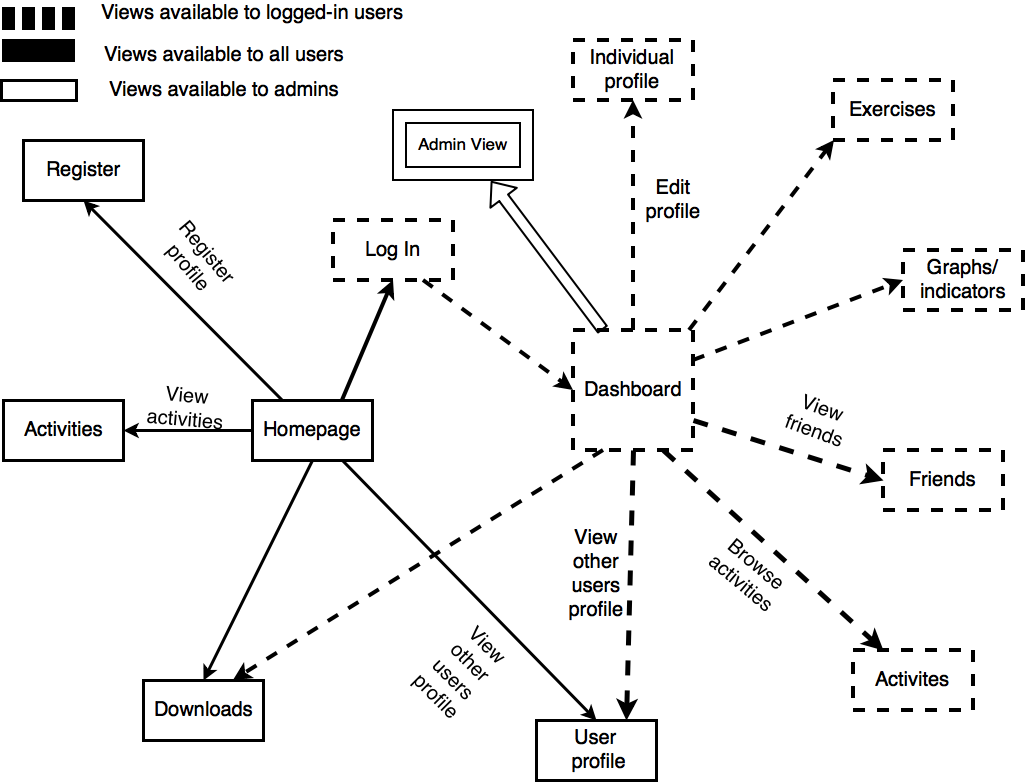
\includegraphics[scale=0.4]{Figures/StateDiagram.png}
\caption{State Diagram of Web Solution}
\label{fig:WebState}
\end{figure}


\subsection{State Diagram of Mobile App?}